\documentclass[10pt]{beamer} 
\usetheme[
%%% options passed to the outer theme
%    hidetitle,           % hide the (short) title in the sidebar
%    hideauthor,          % hide the (short) author in the sidebar
%    hideinstitute,       % hide the (short) institute in the bottom of the sidebar
%    shownavsym,          % show the navigation symbols
%    width=2cm,           % width of the sidebar (default is 2 cm)
    hideothersubsections,% hide all subsections but the subsections in the current section
%    hideallsubsections,  % hide all subsections
    left               % right of left position of sidebar (default is right)
%%% options passed to the color theme
%    lightheaderbg,       % use a light header background
  ]{AAUsidebar} 

% If you want to change the colors of the various elements in the theme, edit and uncomment the following lines
% Change the bar and sidebar colors:
%\setbeamercolor{AAUsidebar}{fg=red!20,bg=red}
%\setbeamercolor{sidebar}{bg=red!20}
% Change the color of the structural elements:
%\setbeamercolor{structure}{fg=red}
% Change the frame title text color:
%\setbeamercolor{frametitle}{fg=blue}
% Change the normal text color background:
%\setbeamercolor{normal text}{bg=gray!10}
% ... and you can of course change a lot more - see the beamer user manual.


\usepackage[utf8]{inputenc}
\usepackage[english]{babel}
\usepackage[T1]{fontenc}
% Or whatever. Note that the encoding and the font should match. If T1
% does not look nice, try deleting the line with the fontenc.
\usepackage{helvet}
\usepackage{listings}
\usepackage{color}
\definecolor{mygreen}{rgb}{0,0.6,0}
\definecolor{mygray}{rgb}{0.5,0.5,0.5}
\definecolor{bluekeywords}{rgb}{0.13,0.13,1}
\definecolor{redstring}{rgb}{0.6,0,0}
\definecolor{javaKeywords}{HTML}{7F0055}
\definecolor{diff}{HTML}{c5c5c5}

\lstdefinestyle{nc}%
{
  %morecomment  = [l]{//},
  morecomment  = [l][\nullfont]{//},
  morecomment  = [is]{/*}{*/}
}

\lstset{ %
  backgroundcolor=\color{white},   % choose the background color; you must add \usepackage{color} or \usepackage{xcolor}
  basicstyle=\scriptsize,        % the size of the fonts that are used for the
  % code
  breakatwhitespace=false,         % sets if automatic breaks should only happen
  % % % at whitespace
  breaklines=true,                 % sets automatic line breaking
  captionpos=b,                    % sets the caption-position to bottom
  commentstyle=\color{mygreen},    % comment style
  deletekeywords={...},            % if you want to delete keywords from the given language
  keepspaces=true,                 % keeps spaces in text, useful for keeping
  columns=flexible,				  % indentation of code (possibly needs columns=flexible)
  language={Java},                 % the language of the code
  numbers=left,                    % where to put the line-numbers; possible values are (none, left, right)
  %numbersep=5pt,                   % how far the line-numbers are from the
  % code
  numberstyle=\tiny\color{black}, % the style that is used for the line-numbers
  showspaces=false,                % show spaces everywhere adding particular underscores; it overrides 'showstringspaces'
  showstringspaces=false,          % underline spaces within strings only
  showtabs=false,                  % show tabs within strings adding particular
  % underscores
  stepnumber=1,                    % the step between two line-numbers. If it's
  % 1, each line will be numbered
  keywordstyle=\color{javaKeywords}\bfseries,
  stringstyle=\color{bluekeywords},     % string literal style
  tabsize=4,                       % sets default tabsize to 2 spaces
  frame=single,
  style=nc,
  framesep=1pt,
  framexleftmargin=3pt,
  literate= {Å}{{\AA}}1 {å}{{\aa}}1 
}

% colored hyperlinks
\newcommand{\chref}[2]{%
  \href{#1}{{\usebeamercolor[bg]{AAUsidebar}#2}}%
}

\setcounter{tocdepth}{1}

\title[ARES]% optional, use only with long paper titles
{ARES}

  % could also be a conference name

\date{\today}

\author[] % optional, use only with lots of authors
{
Jonas Ibrahim\\
Jonathan Magnussen\\
Christoffer Mouritzen\\
\href{mailto:sw609f17@cs.aau.dk}{{\tt sw609f17@cs.aau.dk}}
}
% - Give the names in the same order as they appear in the paper.
% - Use the \inst{?} command only if the authors have different
%   affiliation. See the beamer manual for an example

\institute[
%  {\includegraphics[scale=0.2]{aau_segl}}\\ %insert a company, department or university logo
  Dept.\ of Computer Science\\
  Aalborg University\\
  Denmark
] % optional - is placed in the bottom of the sidebar on every slide
{% is placed on the title page
  Department of Computer Science\\
  Aalborg University\\
  Denmark
  
  %there must be an empty line above this line - otherwise some unwanted space is added between the university and the country (I do not know why;( )
}


% specify a logo on the titlepage (you can specify additional logos an include them in 
% institute command below
\pgfdeclareimage[height=1.5cm]{titlepagelogo}{AAUgraphics/aau_logo_new} % placed on the title page
%\pgfdeclareimage[height=1.5cm]{titlepagelogo2}{graphics/aau_logo_new} % placed on the title page
\titlegraphic{% is placed on the bottom of the title page
  \pgfuseimage{titlepagelogo}
%  \hspace{1cm}\pgfuseimage{titlepagelogo2}
}


\begin{document}
% the titlepage
{\aauwavesbg%
\begin{frame}[plain,noframenumbering] % the plain option removes the sidebar and header from the title page
  \titlepage
\end{frame}}
%%%%%%%%%%%%%%%%

% TOC
\begin{frame}{Agenda}{}
\tableofcontents
\end{frame}

\section{Jonas}
%================================ FRAME 1 ================================
\subsection{Overview}
\begin{frame}{Jonas: Overview}
\begin{itemize}
	\item Introduction:
  		\begin{itemize}
			\item What is GIRAF?
			\item Project Focus
		\end{itemize}
	\item Project Organization:
		\begin{itemize}
			\item Development Methods
			\item Inter-Group Communication
		\end{itemize}
\end{itemize}
\end{frame}
 
%================================ FRAME 2 ================================
\subsection{Project Basics}
\begin{frame}{What is GIRAF?}
\begin{itemize}
	\item Suite of Android Applications
		\begin{itemize}
		    \item Assisting citizens with autism 
  			\item Learning and Planning
  			\item Ongoing since 2011
		\end{itemize}
	\item Multi-Project
		\begin{itemize}
		    \item Collaborative Development 
  			\item Code Maintainence
		\end{itemize}
\end{itemize}
\end{frame}

%================================ FRAME 2 ================================
% \begin{frame}{GIRAF Applications}
% 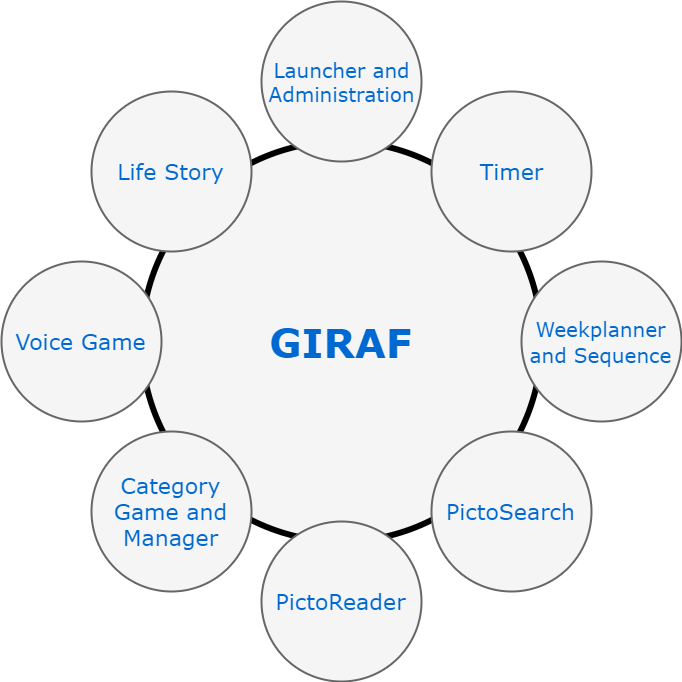
\includegraphics[scale=0.32]{figures/GirafApps.png} 
% \end{frame}

%================================ FRAME 3 ================================
% \begin{frame}{Original State of Giraf}
% \begin{itemize}
% 	\item Front End
% 		\begin{itemize}
% 		    \item Mostly Finished
%   			\item User Testing
%   			\item Occasionally Questionable Design
% 		\end{itemize}
% 	\item Back End
% 		\begin{itemize}
% 		    \item Incomplete
% 		    \item Questionable Quality
% 		    \item Lack of Flexible Database Communication
% 		\end{itemize}
% \end{itemize}
% \end{frame}
% 
% %================================ FRAME 3 ================================
% \begin{frame}{Project Focus}
% \begin{itemize}
% 	\item Finalize Selected Applications
% 	\item Make Changes From User Feedback
% 	\item Implement Usable Database Communication
% \end{itemize}
% \end{frame}

%================================ FRAME 2 ================================
\begin{frame}{Project Focus}
\begin{center}
\begin{minipage}[H]{0.9\linewidth}
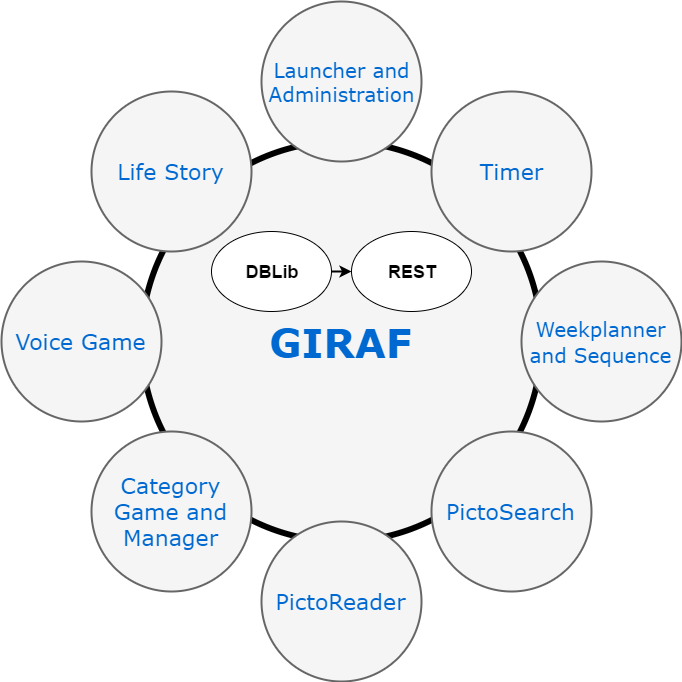
\includegraphics[scale=0.32]{figures/GirafFocus.png} 
\end{minipage}
\end{center}
\end{frame}

%================================ FRAME 2 ================================
\begin{frame}{Our Group's Focus: Login}
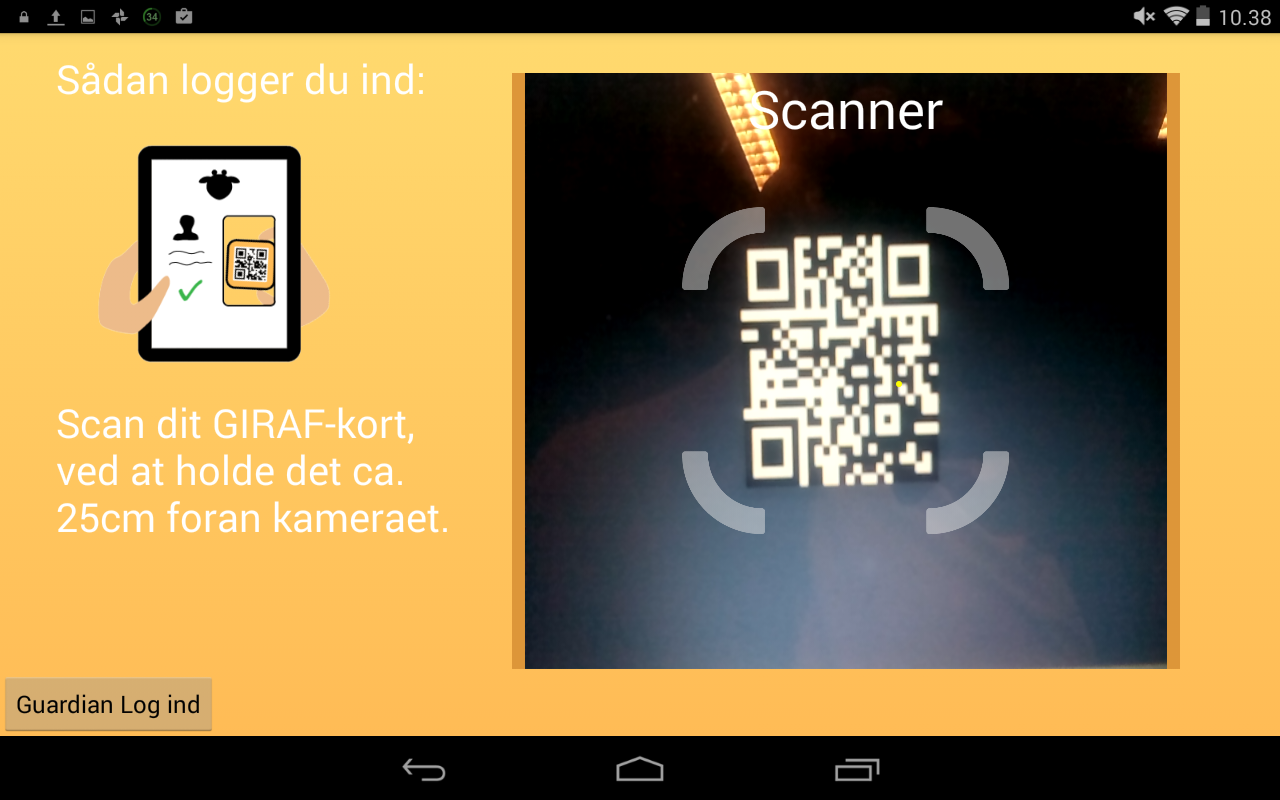
\includegraphics[scale=0.21]{figures/Login.png} 
\end{frame}

%================================ FRAME 2 ================================
\begin{frame}{Our Group's Focus: Main Screen}
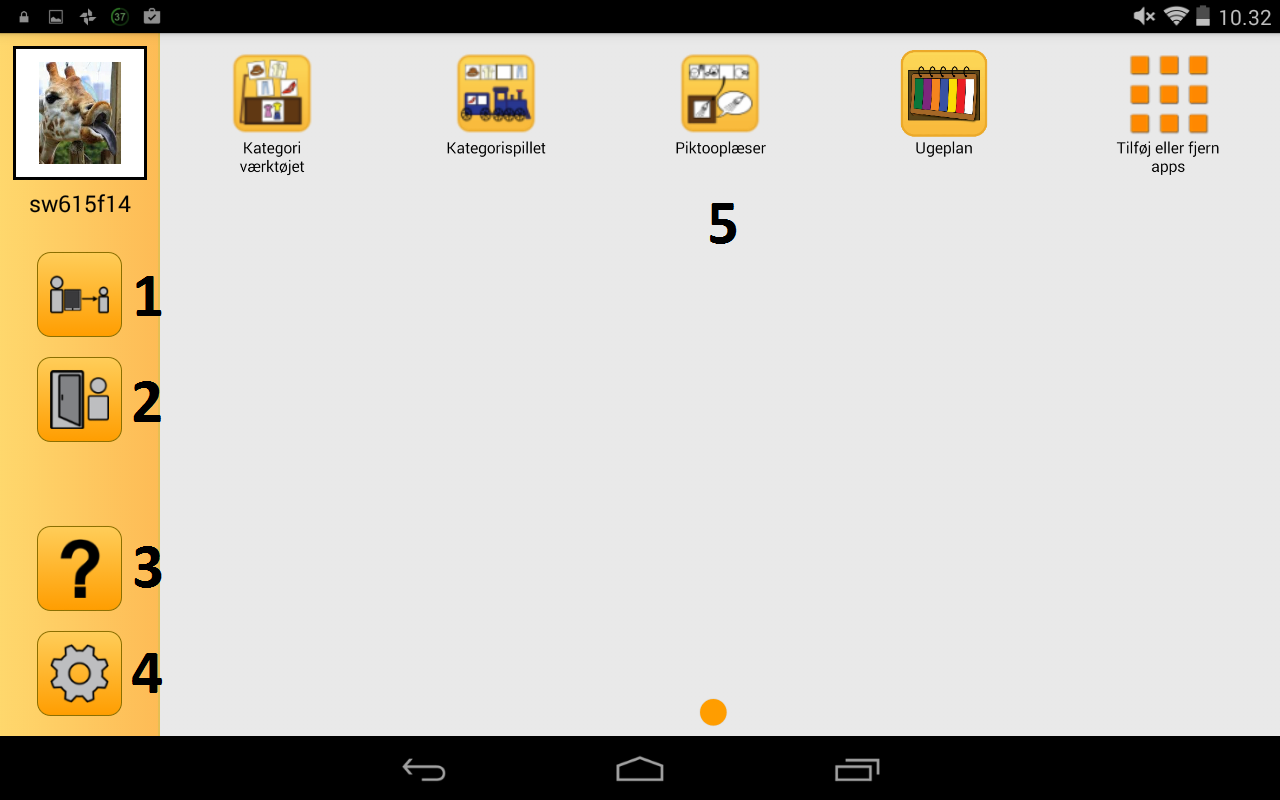
\includegraphics[scale=0.28]{figures/MenuGuardian.png} 
\end{frame}

%================================ FRAME 4 ================================
\subsection{Project Organization}
\begin{frame}{SCRUM of SCRUMS}
\begin{itemize} 
	\item Each Group Organizes Their Own SCRUM
	\item Representative SCRUM Group
	\item Reflection
		\begin{itemize}
		    \item Specialized Agile Approach
		    \item Meetings Too Infrequent
		    \item Discussions Mostly Outside Official Meetings
		\end{itemize}
\end{itemize}
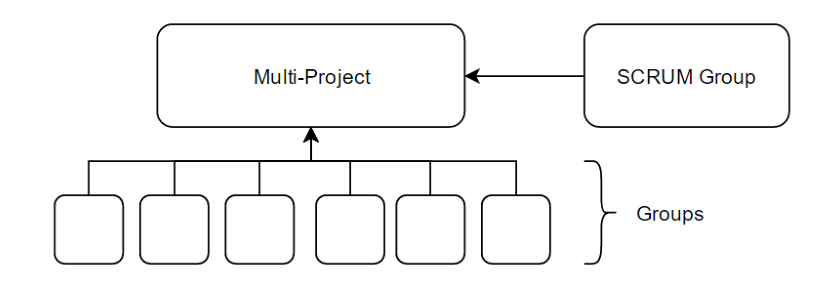
\includegraphics[scale=0.42]{figures/SoS.png} 
\end{frame}

%================================ FRAME 4 ================================
\begin{frame}{Sprint Meetings}
\begin{itemize} 
	\item All Developers Participated 
	\item PO presented user stories
    \item Developers split into groups to brainstorm tasks
	\item Reflection
		\begin{itemize}
		    \item Many People Could Not Contribute
		    \item Some User Stories Were Too General
		    \item Many Tasks Were Added During Sprint
		\end{itemize}
\end{itemize}
\end{frame}

%================================ FRAME 4 ================================
\begin{frame}{General Communiaction}
\begin{itemize} 
	\item Shared Chat Rooms
	\item Close Proximity
	\item Dynamically Planned Meetings
	\item Reflection
		\begin{itemize}
		    \item Difficulty With Unofficial Working Hours
		    \item Some Groups Acting Before Discussing
		    \item Rapid Changes Not Well Communicated
		\end{itemize}
\end{itemize}
\end{frame}

\section{Jonathan}
\subsection{Overview}
\begin{frame}{Jonathan: Overview}
\begin{itemize}
\item Collaborations
\item New Stuff
\end{itemize}
\end{frame}

\subsection{GUI Requirements Analysis}
\begin{frame}{GUI Requirements Analysis}
A collaboration between SW609, SW610 and SW612.\nl

A couple of the more noteworthy questions from the first meeting:
\begin{itemize}
\item How should switching from Guardian to Citizen and back happen?
\item Can there be multiple Guardians pr. Citizen?
\item Who are supposed to login?
\end{itemize}

\end{frame}

\begin{frame]{GUI Requirements Analysis}

A couple of the more noteworthy requirements:

\begin{itemize}
\item There needs to be an option for grayscale.
\item If the system crashes it needs to return to a stable state or return to the Launcher
\item The QR-system needs to be replaced by a password based system.
\item Citizens should not be logged out automatically.
\item There should be an institute type user.
\end{itemize}

Based on the requirements for the users we created this diagram:
\includegraphics[scale=0.5]{figures/LoginDiagram.PNG}

\end{frame}

\subsection{REST Architectural Design}
\begin{frame}{REST Architectural Design}
A Collaboration between SW609, SW610, SW613 and SW615.\nl

\textbf{skal nok rettes lidt til}
The old client/server has serious problems, therefore make a new using the REpresentational State Transfer (REST) model which has the following requirements:
\begin{itemize}
\item Client-Server: Seperate the user interface from data storage and manipulation.
\item Stateless: Each request to the server returns a response which contains all information required for the client to service the request.
\item Cacheable: Responses from the server must implicitly or explicitly declare themselves as either cacheable or not, in order to prevent the client from reusing expired data.
\item Layered System: The client is incapable of determining if it is connected to the main server or an affiliated intermediate entry point.
\item Uniform Interface: The retrieved data is conceptually different from the representation used on the server. Given a set of data, the client should have enough information to edit and delete the respective information of the server.
\end{itemize}
\end{frame}

\begin{frame}{REST Architectural Design}
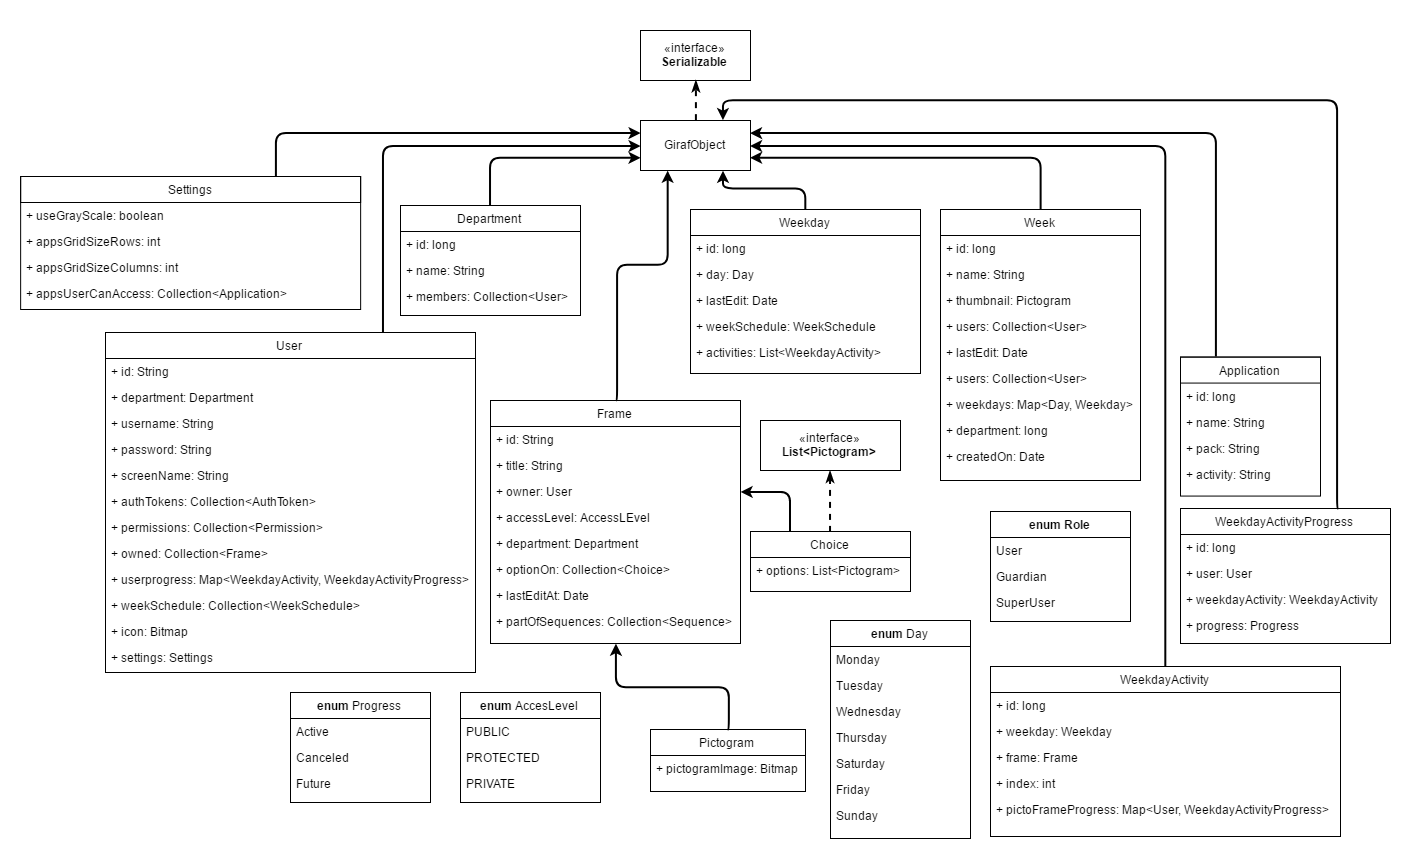
\includegraphics[scale=0.5]{figures/Giraf_RestModelV3.PNG}
\end{frame}

\begin{frame}{REST Architectural Design}

\textbf{WIP}
We use 3 different types of requests:
\begin{itemize}
\item LoginRequest
\item GetRequest
\item PutRequest
\end{itemize}

We also implement VOLLEY which means it is not easy to requests neat.

What is a Request and how do we use it? (hint: RequestQueue and Handler)
\end{frame}

\begin{frame}{REST Architectural Design}
Add a couple of example requests.
\end{frame}

% \subsection{Network Structure}
% \begin{frame}{Network Structure}
% \begin{itemize}
% \item What does the network look like?
% \item Which features are used and how are their domains defined?
% \end{itemize}
% \begin{figure}
%   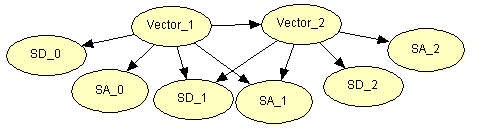
\includegraphics[scale=0.8]{figures/BNDone.PNG}
% \end{figure}
% \end{frame}

\section{Christoffer}
\subsection{Overview}
% \begin{frame}{Christoffer}
% \begin{itemize}
%   \only<1->{\item This}
%   \only<2->{\item is}
%   \only<3->{\item a}
%   \only<4>{\item test}
% \end{itemize}
% \end{frame}

\begin{frame}{Christoffer: Overview}
\begin{itemize}
  \item Technical Details
  		\begin{itemize}
  			\item How was REST implemented
  			\item The impact of the REST implementation
  			\item Asynchronous requests and the problems they cause
  			\item Request chaining
  			\item The settings problem	  
		\end{itemize}
  \item Future work
  		\begin{itemize}
  			\item Activity controllers
  			\item General Component lib
  			\item General Launcher
		\end{itemize}
  \item Showcase the Launcher
\end{itemize}
\end{frame}

\subsection{Technical Details}
\begin{frame}{Technical Details}
\begin{itemize}
  \item Main
  \item Track
  \item GetDataAndCalculate
  \item WaitAndFire
\end{itemize}
\end{frame}

\begin{frame}[fragile]{Main}
\only<1>{
\begin{itemize}
  \item Purpose
  	\begin{itemize}
  		\item Start tasks
  		\item Setup
  	\end{itemize}
  \item Key implementation points
  	\begin{itemize}
  		\item Setup sensors / camera
  		\item Start tasks
	\end{itemize}
\end{itemize}
}
\begin{onlyenv}<2>
\begin{itemize}
  \item Key implementation points
  	\begin{itemize}
  		\item Setup sensors / camera
  		\item Start tasks
	\end{itemize}
\end{itemize}
\begin{center}
\begin{minipage}[H]{0.9\linewidth}
\begin{lstlisting}
PosRegEnable(ROTATE_MOTOR);
PosRegEnable(ANGLE_MOTOR);
SetMotorRegulationTime(10);
NXTCam_Init(CAM_PORT, CAM_ADDR);
NXTCam_SendCommand(CAM_PORT, CAM_ADDR, 'A'); 
NXTCam_SendCommand(CAM_PORT, CAM_ADDR, 'E');
SetSensorUltrasonic(SENSOR_LEFT);
SetSensorUltrasonic(SENSOR_RIGHT);
Precedes(Track,GetDataAndCalculate);
\end{lstlisting} 
\end{minipage}
\end{center}
\end{onlyenv}
\end{frame}

\begin{frame}[fragile]{Track}
\only<1>{
\begin{itemize}
  \item Purpose
  	\begin{itemize}
  		\item Track targets
  		\item Information sharing
  	\end{itemize}
  \item Key implementation points
  	\begin{itemize}
  		\item Camera interaction
  		\item Target present
  		\item Determin Direction
  		\item Turn turret 
	\end{itemize}
\end{itemize}
}
\begin{onlyenv}<2>
\begin{itemize}
  \item Key implementation points
  	\begin{itemize}
  		\item Camera interaction
  		\item Target present
  		\item Determine Direction
  		\item Turn turret 
	\end{itemize}
\end{itemize}
\begin{center}
\begin{minipage}[H]{0.9\linewidth}
\begin{lstlisting}
while(track){
	NXTCam_GetBlobs(CAM_PORT, CAM_ADDR, nblobs, bc, bl, bt, br, bb);
    if(nblobs > 0){
    	blobInCam = true;
        ....
        if(lib_direction != NO_DIRECTION){
        	tempSpeed = GetSpeed(blobCenter );
            if(tempSpeed > 0 && lib_direction == RIGHT_DIRECTION)
            	OnFwd(ROTATE_MOTOR, tempSpeed);
            else if(tempSpeed < 0 && lib_direction == LEFT_DIRECTION)
            	OnFwd(ROTATE_MOTOR, tempSpeed);
        }
	}else{
    	blobInCam = false;
        ...
    	Off(ROTATE_MOTOR);
	}
    DetermineDirection(blobCenter, oldBlobCenter, directionCount);
}
\end{lstlisting} 
\end{minipage}
\end{center}
\end{onlyenv}
\end{frame}

\begin{frame}[fragile]{GetDataAndCalculate}
\only<1>{
\begin{itemize}
  \item Purpose
  	\begin{itemize}
  		\item Collect data
  		\item Calculate vectors and positions
  		\item Determine the shooting position
  	\end{itemize}
	\item Key implementation points
		\begin{itemize}
  			\item Busy wait 
  			\item Make position data
  			\item Calculate fire position 
		\end{itemize}
\end{itemize}
}
\begin{onlyenv}<2>
\begin{itemize}
	\item Key implementation points
		\begin{itemize}
  			\item Busy wait 
  			\item Make position data
  			\item Calculate fire position 
		\end{itemize}
\end{itemize}
\begin{center}
\begin{minipage}[H]{0.9\linewidth}
\begin{lstlisting}
while(collecting){
	if(blobInCam){
        if(length != NO_DATA){
            if(MakePosData(length,GetMotorAngle(),CurrentTick(),tempPosData)){
            	posData[posDataCounter] = tempPosData;
                posDataCounter++;
            }
            if(posDataCounter == DATASETS_NEEDED_TO_CALCULATE){
				track = false;
                Off(ROTATE_MOTOR); 
                StopTask(Track);
                DirectionVector vector = CalcDirVector(posData,posDataCounter);
                fire = CalcFireData(CalcFuturePos(vector,MILLISECONDS_TO_HIT));
                StartTask(WaitAndFire);
            }
    	}
	}
}
\end{lstlisting} 
\end{minipage}
\end{center}
\end{onlyenv}
\end{frame}

\begin{frame}[fragile]{WaitAndFire}
\only<1>{
\begin{itemize}
  \item Purpose
  	\begin{itemize}
  		\item Wait until the calculated time
  		\item Shoot the target at the calculated position
  		\item Reset the turret
  	\end{itemize}
  \item Key implementation points
  	\begin{itemize}
  		\item Stop GetDataAndCalculate
  		\item Load / Rotate and Angle
  		\item Busy wait to fire
  		\item Reset / Start tasks 
	\end{itemize}
\end{itemize}
}
\begin{onlyenv}<2>
\begin{itemize}
  \item Key implementation points
  	\begin{itemize}
  		\item Stop GetDataAndCalculate
  		\item Load / Rotate and Angle
  		\item Busy wait to fire
  		\item Reset / Start tasks 
	\end{itemize}
\end{itemize}
\begin{center}
\begin{minipage}[H]{0.9\linewidth}
\begin{lstlisting}
collecting = false;
LoadRound();
Off(ROTATE_MOTOR);
RotateH(fire.angleH);
Angle(fire.angleV);
while(true){
	if(CurrentTick() >= fire.timeToHit && !alreadyFired){
    	alreadyFired = true;
        Fire();
        break;
    }
}
Angle(START_ANGLE);
...
Wait(4000);
StartTask(Track);
StartTask(GetDataAndCalculate);
\end{lstlisting} 
\end{minipage}
\end{center}
\end{onlyenv}
\end{frame}
{\aauwavesbg
\begin{frame}[plain,noframenumbering]
  \finalpage{Thank you!}
\end{frame}}
%%%%%%%%%%%%%%%%

\end{document}
